%\documentclass[tikz,border=5mm,convert={outfile=\jobname.png}]{standalone}
\documentclass[tikz,border=5mm]{standalone}
\usepackage[utf8]{vietnam}
\usepackage{tikz}
\usetikzlibrary{calc}
\usepackage[nodayofweek]{datetime}
%=============
\begin{document}
	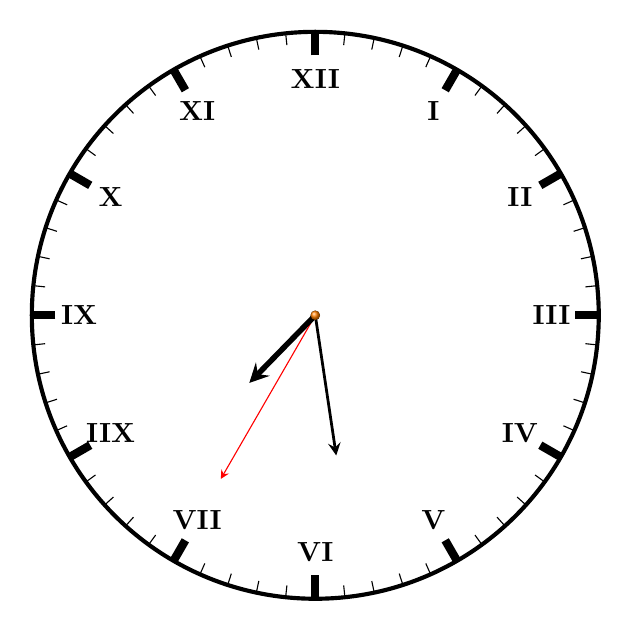
\begin{tikzpicture}[>=stealth]
		\def\r{3}%Bán kính đường tròn hiển thị giờ
		\def\gio{\the\currenthour}%Nhập giờ
		\def\phut{\the\currentminute}%Nhập phút
		\def\giay{35}%Nhập giây
		% \path node{\the\currenthour:\the\currentminute};
		\foreach \i/\j in {60/I,30/II,0/III,-30/IV,-60/V,-90/VI,-120/VII,-150/IIX,-180/IX,-210/X,-240/XI,-270/XII}{\draw (\i:\r) node{\bf \j};}%Chữ hiển thị giờ
		\foreach \i in {1,...,60}{
			\draw (\i *6: 1.15*\r)--(\i *6: 1.2*\r);
			% \draw (90-\i *6:1.3*\r) node[scale=0.5] {$\i$};
		} %Vạch chia giây và số hiển thị bên ngoài
		\foreach \i in {0,30,...,330}{\draw[line width=3] (\i:1.1*\r)--(\i:1.2*\r);}%Vạch chia giờ
		\draw[line width=1.5] (0:0) circle (1.2*\r);%Đường tròn bao quanh vạch chia giờ
		\pgfmathsetmacro{\gocgio}{90-(\gio *30+\phut /2+0.5*\giay/60)}%Tính góc kim giờ
		\pgfmathsetmacro{\gocphut}{90-(\phut *6+\giay *0.1)}%Tính góc kim phút
		\pgfmathsetmacro{\gocgiay}{90-\giay *6}%Tính góc kim giây
		\draw[->,red] (0:0)--(\gocgiay:0.8*\r);%Vẽ kim giây
		\draw[line width=1,->] (0:0)--(\gocphut:0.6*\r);%Vẽ kim phút
		\draw[line width=2,->] (0:0)--(\gocgio:0.4*\r);%Vẽ kim giờ
		\fill[ball color=orange ](0:0) circle (0.02*\r);%Vẽ tâm đồng hồ
	\end{tikzpicture}
	%============
\end{document}